\chapter{DTLS} \label{Chp: DTLS}

In this chapter we analyse DTLS on Contiki. We consider only two ciphersuites those have been implemented by the tinydtls implementation, which are TLS\_PSK\_WITH\_AES\_128\_CCM\_8 and TLS\_ECDHE\_ECDSA\_WITH\_AES\_128\_CCM\_8. 

One thing to be noticed is that both ciphersuites uses AES-128 CCM for data encryption and therefore they only behave different during handshake. Hence we do not distinguish application data encrypted by both ciphersuites.

\section{Protocol and Implementation}

Due to the fact that tinydlts implemented only a minimum features of DTLS and supports only two ciphersuites, TLS\_PSK\_WITH\_AES\_128\_CCM\_8 and TLS\_ECDHE\_ECDSA\_WITH\_AES\_128\_CCM\_8, we have found no applicable attacks from \cite{rfc7457}.

\section{DTLS Handshake}

\textbf{[To be done...]}

\section{Packet Size}

Since application data are encrypted using AES-128 CCM, its size is not hidden and is visible in the header, as highlighted in the middle of \Cref{Fig: Size of application data in DTLS}.

\begin{figure*}[ht!]
	\center
	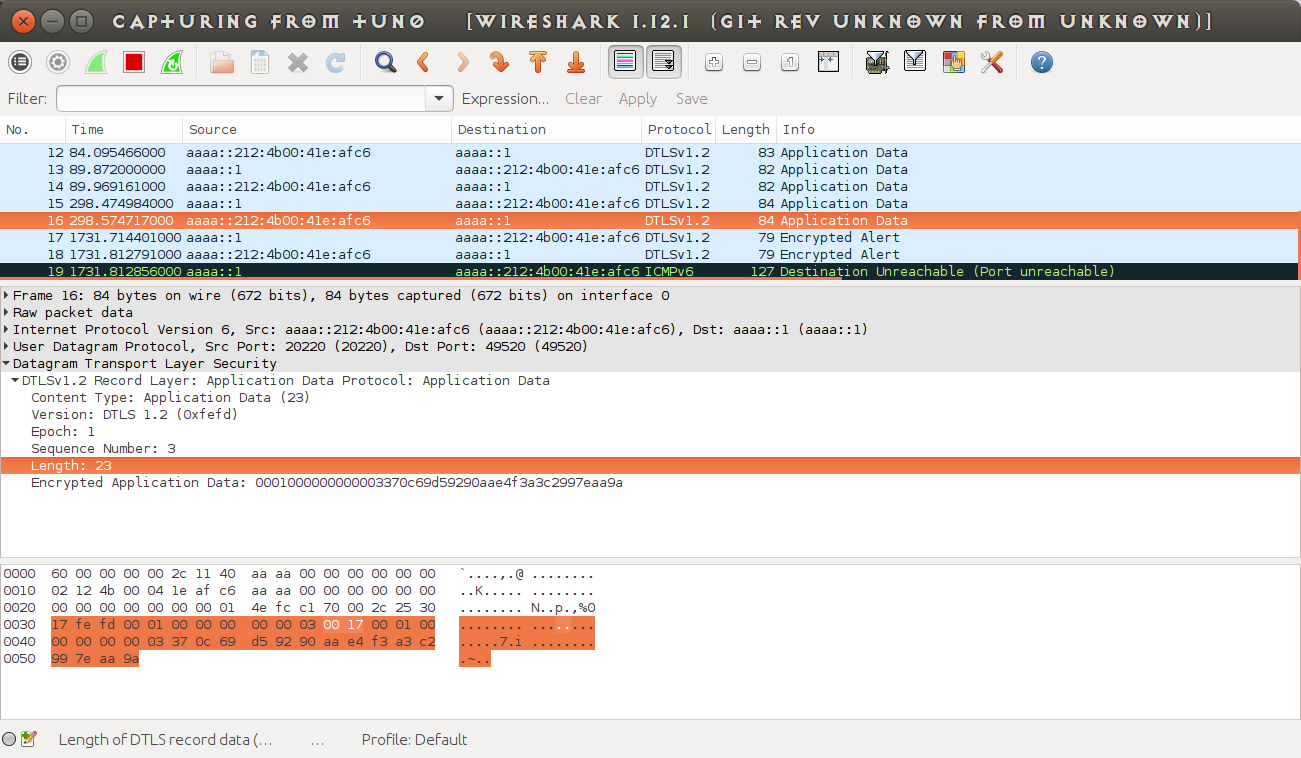
\includegraphics[width=.7\textwidth]{fig/dtlslength.png}
	\caption{Size of application data in DTLS}
	\label{Fig: Size of application data in DTLS}
\end{figure*}

Referring to \cite{rfc5116}, the size of application data is exactly the value of the highlighted Length in \Cref{Fig: Size of application data in DTLS} minus $16$ bytes.

%CoAP

\section{Timing}

In this section, we analyse the availability of timing information when the application data is protected by DTLS using the tinydtls implementation on Contiki.

\subsection{Processing Model}

The procedure of a Session with DTLS is as depicted by \Cref{Fig: A Session with DTLS}.

\begin{figure*}[ht!]
	\center
	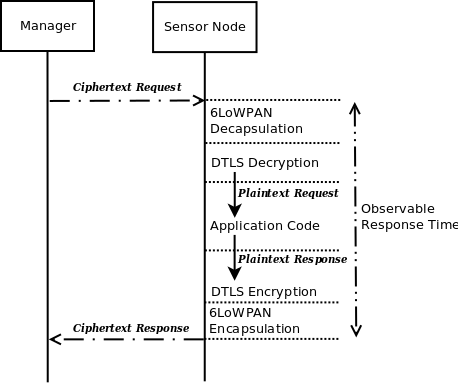
\includegraphics[width=0.8\textwidth]{fig/dtls_session.png}
	\caption{A Session with DTLS}
	\label{Fig: A Session with DTLS}
\end{figure*}

DTLS provides protection between only two Sensor Nodes in the network; thus the source and destination are consistent within a DTLS session. The 6LoWPAN encapsulation and decapsulation procedure are hence identical for all packets using the same DTLS session; therefore the time length of 6LoWPAN decapsulation and encapsulation in \Cref{Fig: A Session with DTLS} are considered to be constant.

Therefore in this section we put our interest in the timing of DTLS decryption/encryption and the execution time of application code.

\subsection{AES Timing} \label{tinydtls AES Timing}

tinydtls uses the OpenBSD optimised AES implementation. Its source code is available at:\\ 
\url{https://github.com/Salties/MyRepository/blob/master/tinydtls-0.8.2/aes/rijndael.c}

We applied the same tests as described in \Cref{Sec: AES Timing}. 

The average AES execution time is shown in \Cref{Tbl: tinydtls AES execution time estimation}.

\begin{table}[ht!]
	\center
	\begin{tabular}{|c|c|}
		\hline
		                        & CC2538 SW \\ \hline
		50 executions           & 160.07          \\ \hline
		100 executions          & 320.06          \\ \hline
		150 executions          & 480.05          \\ \hline
		200 executions          & 640.13          \\ \hline
		Ticks per executions    & 3.20            \\ \hline
		AES Execution Time (ms) & 0.098           \\ \hline
	\end{tabular}
	\caption{tinydtls AES execution time estimation}
	\label{Tbl: tinydtls AES execution time estimation}
\end{table}

The result of Fixed vs Random test is shown in \Cref{Tbl: Fixed vs Random test result for tinydtls AES execution time on CC2538}

\begin{table}[ht!]
	\center
	\begin{tabular}{|c|c|c|}
		\hline
		                         & Fixed       & Random      \\ \hline
		Sample Mean              & 640.28      & 640.25      \\ \hline
		Sample Standard Deviation & 0.49        & 0.53        \\ \hline
		t-score                  & \multicolumn{2}{c|}{1.32} \\ \hline
	\end{tabular}
	\caption{Fixed vs Random test result for tinydtls optimised AES execution time on CC2538. Executions per sample: $200$. Sample size: $1000$.}
	\label{Tbl: Fixed vs Random test result for tinydtls AES execution time on CC2538}
\end{table}

Applying the TVLA t-score threshold which is $4.5$, the results in \Cref{Tbl: Fixed vs Random test result for tinydtls AES execution time on CC2538} imply that the tinydtls optimised AES implementation has passed our test, i.e. no leakage is detected through the execution time of the tinydtls optimised AES implementation. 

The result is consistent with our expectation, as the implementation has no branch\footnote{The only branch in the source code is for AES-192 and AES-256, which are not used in the ciphersuites.} in the source code and is done with only statements of assignment, shift and XORs. The low sample standard deviation is also an evidence that supports our expectation that the AES implementation takes a nearly constant time.

The source code and data for our tinydtls AES timing experiments are available at: \\
\url{https://github.com/Salties/MyRepository/tree/master/experiments/dtlsaes} \\
and \\
\url{https://github.com/Salties/MyRepository/tree/master/experiments/dtlsaes/Data}

\subsection{Protocol Suite Processing Timing}

Since the AES implementation takes a nearly constant time, its impact to the timing information induced by different session keys is therefore can be considered negligible. 

We estimated the overall processing time of the protocol suite\footnote{6LoWPAN and DTLS processing in \Cref{Fig: A Session with DTLS}.} by using an application which the Sensor Node responses with a constant predefined value. A hint of the source code is shown in \Cref{nullapp}.

\lstinputlisting[label={nullapp}, captionpos=b, caption={Application code with negligible execution time}]{src/nullapp.c} 

There is no actual code being executed in the application showed in \Cref{nullapp}. The execution time of this application code can be considered negligible and hence the observable response time between Request and Response in \Cref{Fig: A Session with DTLS} can therefore viewed as an approximation of the overall protocol suite processing time.

Without exceeding 802.15.4 MTU, the length of DTLS Payload is ranged from $1$ byte to $47$ bytes. However in our setup, the Requests are retransmitted by the border router and thus one byte is taken by the decompressed Hop Limit in IPv6 Header. We experimented with combinations of Requests ranging from $1$ byte to $46$ bytes and Responses ranging from $1$ byte to $47$ bytes. We denote $|Req|$ and $|Res|$ as the length in bytes of the DTLS Payload in Requests and Responses respectively.

\Cref{Fig: Example histograms of protocol suite processing time on CC2538 with DTLS} shows two example histograms of part of our results on CC2538.

\begin{figure}[ht!]
	\center
	\begin{subfigure}{.4\textwidth}
	\center
	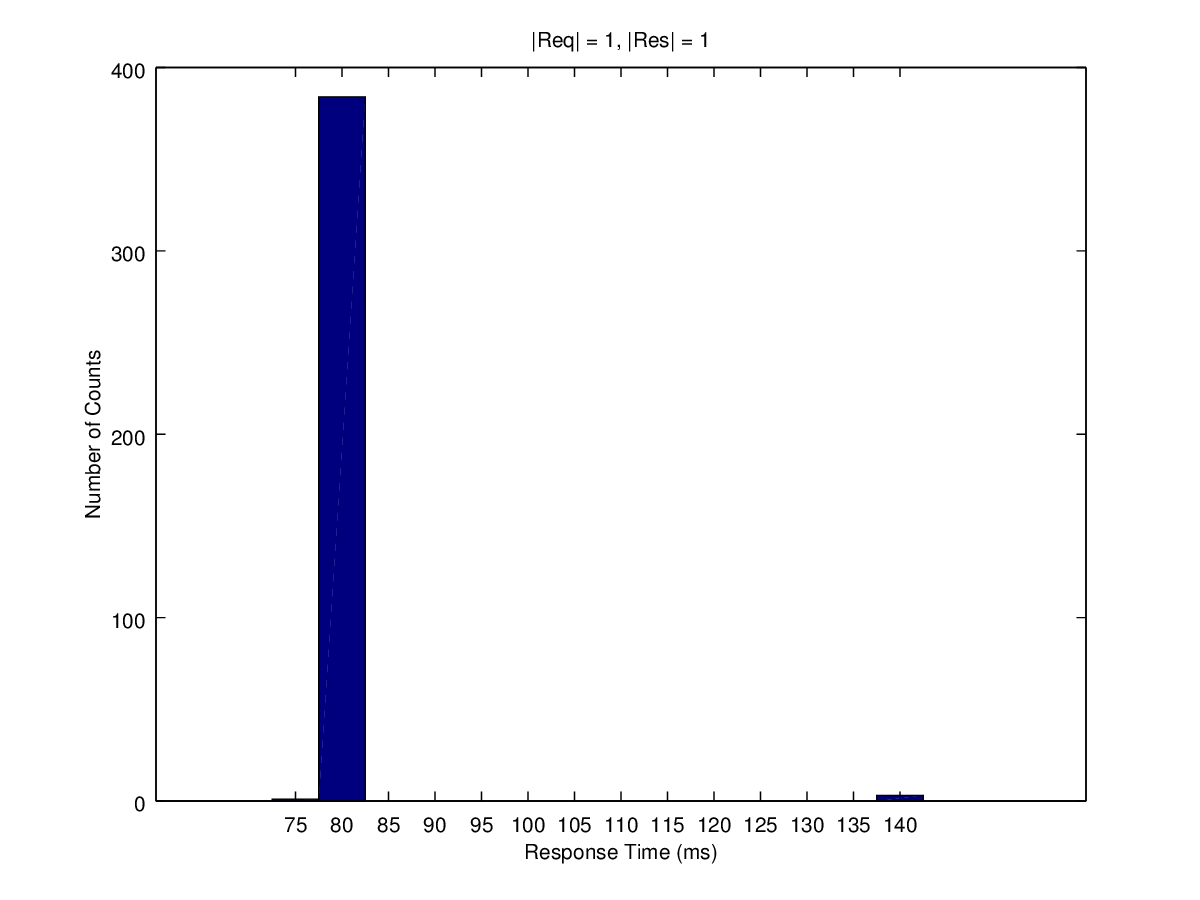
\includegraphics[width=\linewidth]{fig/dtlstimehist_min.png}
	\end{subfigure}
	\begin{subfigure}{.4\textwidth}
	\center
	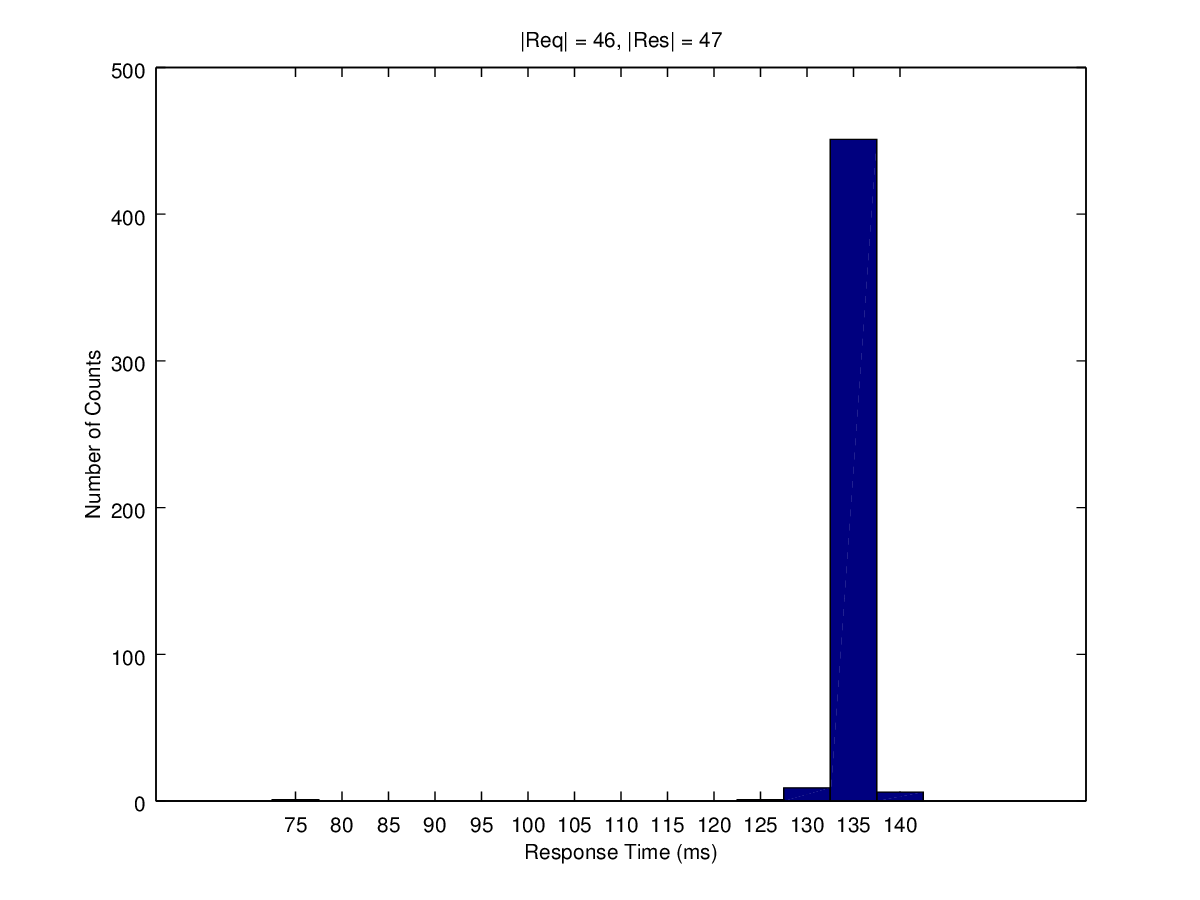
\includegraphics[width=\linewidth]{fig/dtlstimehist_max.png}
	\end{subfigure}
	\caption{Example histograms of protocol suite processing time on CC2538 with DTLS}
	\label{Fig: Example histograms of protocol suite processing time on CC2538 with DTLS}
\end{figure}

Similar to the ECHO response time we have shown in \Cref{Fig: Histograms of ECHO response times on different setups}, the response times in these experiments also appears to densely cluster near a specific value while a few are drifted away; hence we use their sample median to characterise the protocol suite processing time. The medians of the examples shown in \Cref{Fig: Example histograms of protocol suite processing time on CC2538 with DTLS} are summarised in \Cref{Tbl: Median of response times in examples}. It is clear that the response time of Request and Response at their maximum length is significantly longer comparing to Request and Response at their minimum length.
 
\begin{table}
	\center
	\begin{tabular}{|c|c|c|}
		\hline
		 				&($|Req|$ == 1, $|Res|$ == 1) 	& ($|Req|$ == 46, $|Res|$ == 47) 	\\ \hline
		 Sample Median	&79.712 ms                  			& 132.740 ms                   			\\ \hline
	\end{tabular}

	\caption{Medians of response time in the examples of \Cref{Fig: Example histograms of protocol suite processing time on CC2538 with DTLS}}
	\label{Tbl: Median of response times in examples}
\end{table}

Further more, our data also shows that both $|Req|$ and $|Res|$ are linear related to the response time.

\begin{figure}[ht!]
	\center
	\begin{subfigure}{0.45\textwidth}
	\center
	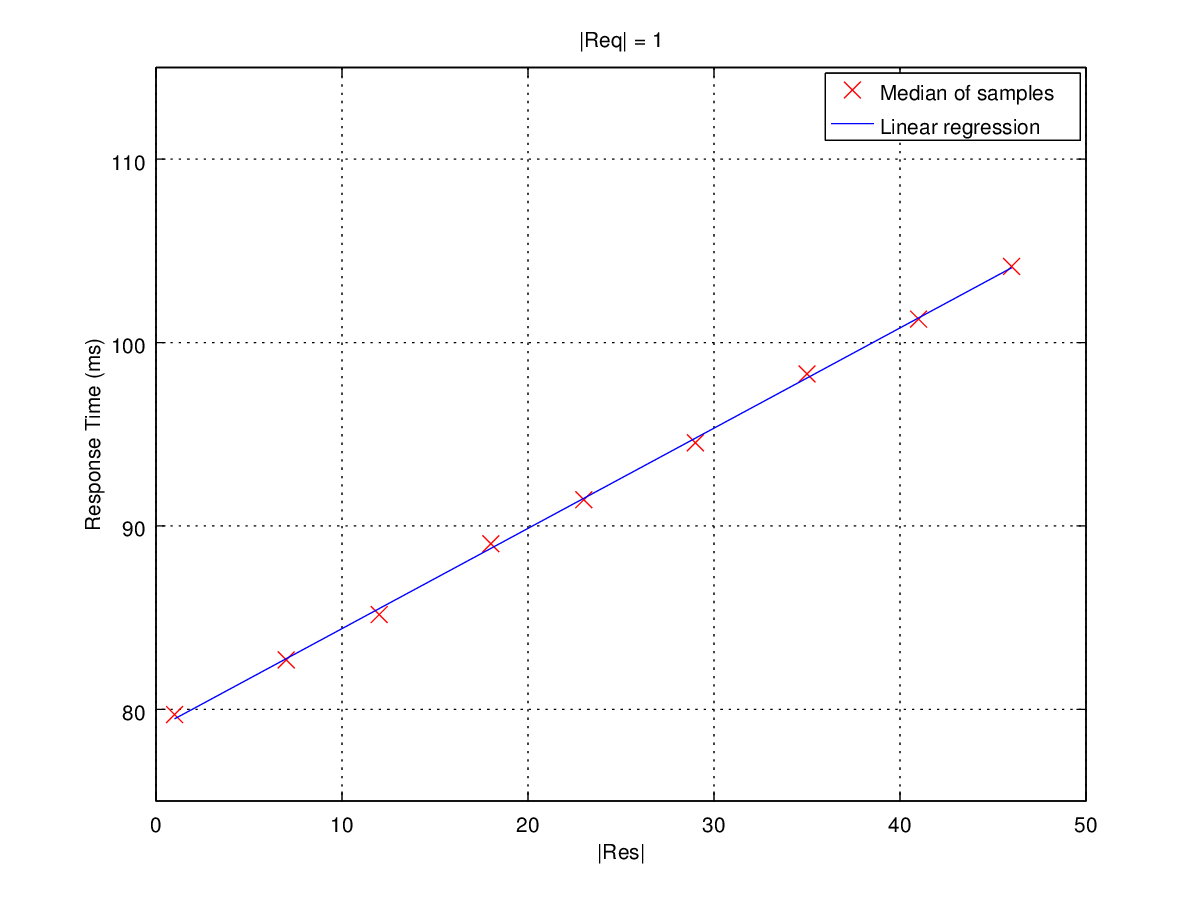
\includegraphics[width=\textwidth]{fig/dtlstime_req1.png}
	\subcaption{$|Req| = 1$, variable $|Res|$}
	\end{subfigure}
	\begin{subfigure}{0.45\textwidth}
	\center
	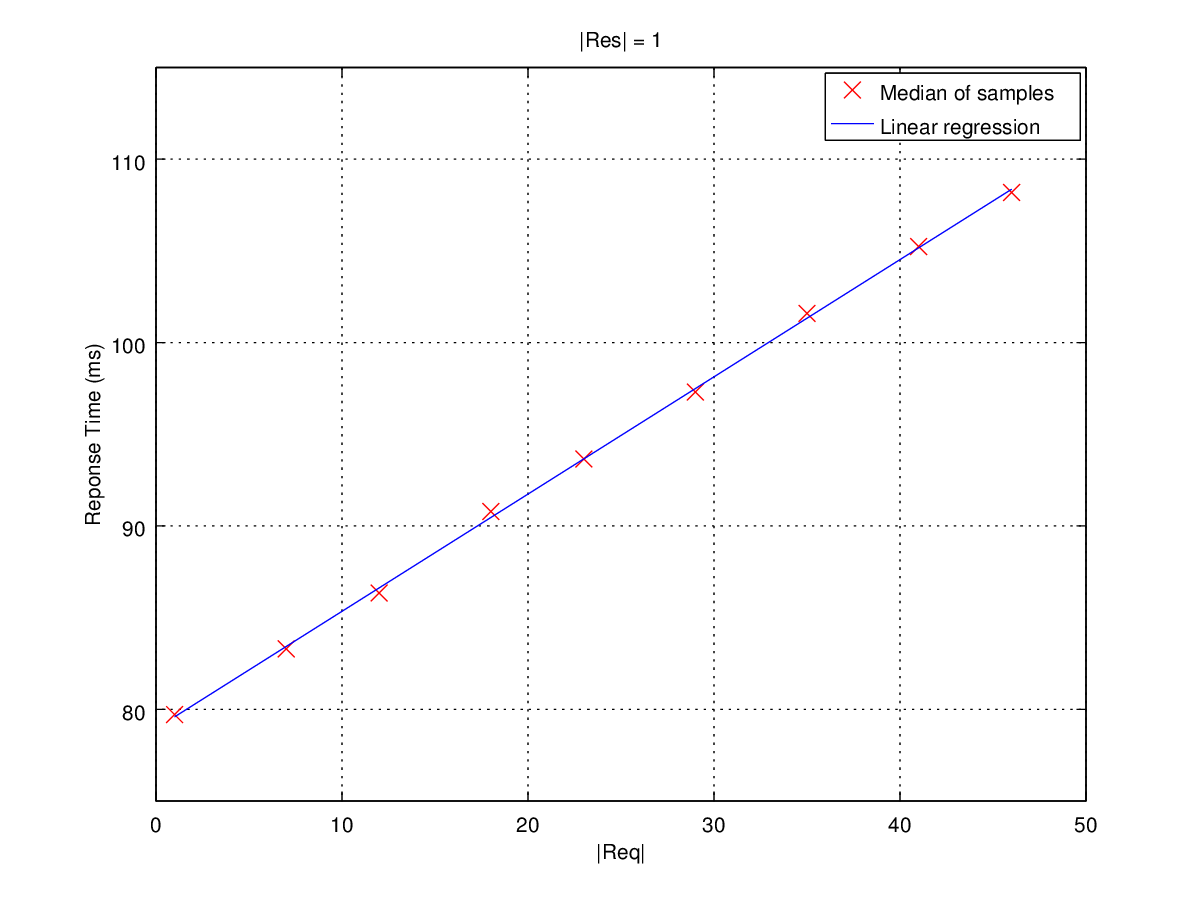
\includegraphics[width=\textwidth]{fig/dtlstime_res1.png}
	\subcaption{Variable $|Req|$, $|Res| = 1$}
	\end{subfigure}
	\caption{Protocol suite processing time on CC2538 with DTLS}
	\label{Fig: Protocol suite processing time on CC2538 with DTLS}
\end{figure}

\subsection{Application Code Timing}




%DTLS has potentially the best interoperability as it is an variation of the widely used TLS in Internet. However, its design might not fit into the nature of WSN for practical reasons.
%
%\section{Implementation Issues}
%The most practical implementation we found on Contiki OS so far is tinydtls.
%
%tinydtls\cite{tinydtls} currently supports two ciphersuites, namely TLS\_PSK\_WITH\_AES\_128\_CCM\_8 and TLS\_ECDHE\_ECDSA\_WITH\_AES\_128\_CCM\_8. 
%
%However, we encountered several difficulties when trying to set up an encrypted network using tinydtls.
%
%\begin{description}
%\item[Low Computational Power] \hfill \\
%Curve computation requires relatively a large amount of computational power. Even using a relatively powerful platform (CC2538), it still takes minutes to complete a DTLS handshake with
%TLS\_ECDHE\_ECDSA\_WITH\_AES\_128\_CCM\_8.
%
%\item[Low Bandwidth] \hfill \\
%The 6LowPAN standard specifies that the minimum MTU is 127 bytes whilst 67 (87 with LLSEC) bytes are occupied by protocol headers until UDP, which leaves 60 (40 with LLSEC) bytes available for UDP layer payload. This value has been exceeded by several handshake packets even with pre-shared keys. Doing key exchange or even using longer keys only makes this problem worse. Some attempts have been made to solve this issue, e.g. CoDTLS\cite{CoDTLS}\footnote{This draft has been abandoned for some reason we do not know.}. As a result, DTLS is only available on those devices support extra frame length than 6LowPAN requirements.
%
%\item[Code Size] \hfill \\
%The tinydtls fails to fit into some devices, e.g. skymote, as its size of code is too large.
%\end{description}
%
%Therefore although TLS\_PSK\_WITH\_AES\_128\_CCM\_8 is less flexible (and probably less secure) as it uses a pre-shared master secret, it is still considered to be a relatively practical security measure as it requires less resources.
%
%\section{No Multicast Support}
%Some application protocols, such as CoAP, utilises the multicast feature of 6LowPAN whilst TLS is a protocol designated for securing communications between two parties, so is DTLS. To  our knowledge, DTLS does not make any attempt to support multicasting.
%
%\section{Overloading DTLS with LLSEC}
%Adopting both security measures at the same time is possible as they are implemented at different layers. However, it is questionable whether this will bring more security, as both {\it noncoresec} and TLS\_PSK\_WITH\_AES\_128\_CCM\_8 are using 128 bit AES with CCM mode as their cryptographic primitive.
